
\title{Software Processes Assignment One}
\author{Alastair Mory 21120848}
\date{September 8, 2019}


\documentclass[12pt,a4paper]{article}
\usepackage[margin=1in]{geometry}

\usepackage{amsmath}

\usepackage{graphicx}
\graphicspath{ {./fig/} }

\begin{document}
	\begin{titlepage}
		\clearpage\maketitle
		\thispagestyle{empty}
		\tableofcontents
		\newpage

	\end{titlepage}
	
	\section{Background}

		This report will attempt to model the software validation process in order to help determine appropriate benchmarks and resource allocation for the team testers working to validate the system in our current project.
	
		The system validation process in software engineering can be conceptualised as a paradigm involving two sub-processes: fault finding and fault resolution, this paradigm will be used to aid the analysis.
	
		The team available to work on testing the system and fixing bugs consists of three software engineers each working 25 hours per week.
	
	

	\section{Defect Detection}
	
% Explain how you performed curve fitting on the data. What software did you use, and did you have to make any assumptions? What models did you select?
% For each model:
% Give the generic equation for the model
% State the values of the parameters as you have estimated them
% Include a chart showing a plot of the defect data and your fitted curve
% Give the goodness of fit measure you have calculated, and an English explanation of what it means (is this a good fit, or not?)
% Use the model to estimate the total number of defects in the past project, and how many remain after the 300 known defects are fixed, and explain how you did so
% Describe any assumptions required for making the estimation, and any limitations.
% State which model you think is most plausible for the data, and why.
	
		Data has been collected from a previous similar project with 300 known defects.
		This data contains an approximate time frame of when the defects were found (how many weeks it took a single tester working 25 hours per week to find them). Each defect is categorised by its impact to the project (major or minor) and expected effort needed to resolve it (hard or easy) resulting in four classes of defect: major hard, major easy, minor hard and minor easy.
		

		\begin{figure}[h]
			\centering
			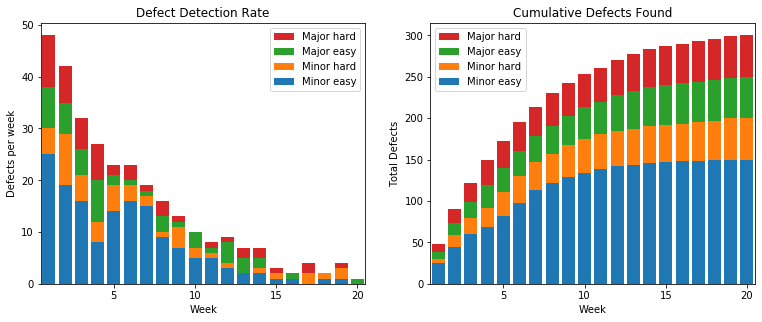
\includegraphics[scale=0.6]{histogram}
			\caption{Defect detection data}
		\end{figure}

		
		\ \\
		
		%% Assumptions and Curve fitting process %%
		Figure 1 shows the defect detection rate against week closely resembles an exponential decay function, i.e. it approximately fits an equation of the form:
		\[
			y = ae^{-bx}
		\]
		Which can be linearised to:
		\[
			log(y) = log(a) - b x
		\]
		Three equations modelling the defect detection rate are discussed below; defects by type
		
		Each model below assumes some form of exponential function for the rate of defect detection. The first two use a logarithmic function to linearise the data and apply SciPy's \texttt{stats.linregress} method for a linear regression, while the third uses the \texttt{optimize.curve\_fit} method to directly fit an exponential decay regression.
		
		%% Goodness of fit and AUC calculation %%
		In each model the goodness of fit is described by the correlation coefficient and standard error. The correlation coefficient, or $R^2$ gives the proportion of the variance in the data that is explained by the fitted curve, while the standard error is the standard deviation of the residuals in the data (the difference between the fitted curve and each data point).
		
	\subsection{Defects by Type (Log Linear)}
		This first model (figure 2) involves separate exponential decay regressions for each defect type giving a fitted function of the form:
		
		\[
			y = a_1 e ^ {-b_1 x_1}  
			  + a_2 e ^ {-b_2 x_2} + a_3 e ^ {-b_3 x_3} + a_4 e ^ {-b_4 x_4}
		\]		
		
		Where $x_1, x_2, x_3$ and $x_4$ are the major hard, major easy, minor hard and minor easy defects respectively. A linear least-squares regression was performed individually for each defect type, yielding the following equations:
		\begin{align*}
			\text{Major Hard } &= 6.13 e ^ {-0.124 x}\\
			\text{Major Easy } &= 6.00 e ^ {-0.119 x}\\
			\text{Minor Hard } &= 5.99 e ^ {-0.115 x}\\
			\text{Minor Easy } &= 36.29 e ^ {-0.211 x}
		\end{align*}
		
		\begin{figure}[hh]
			\centering
			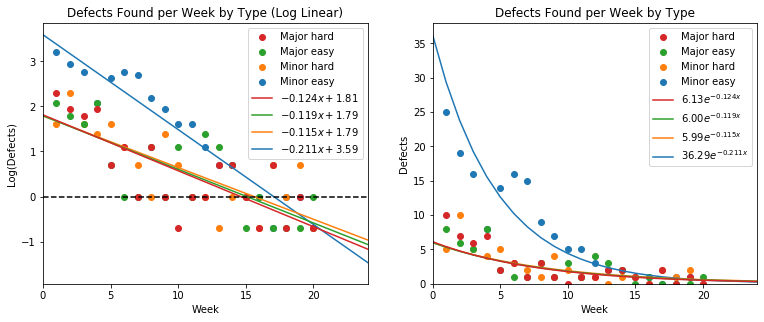
\includegraphics[scale=0.6]{type_log_lin}
			\caption{Defect detection data, defects by individual type log linear regression.}
		\end{figure}
		
		Modelling the defect discovery rate separately for each defect type results in a average fit too the data, as correlation coefficient varies from 0.55 (major easy) to 0.8 (minor easy) with a standard of error of between 1.4 (minor hard) and 3.2 (minor easy).\\
		
		When these equations are combined their integral from 0 to infinity gives an estimate for the total bugs in the system of roughly 324, or 24 unfound defects remain:\\
		
		\[
		\int_0^\infty 6.13e^{-0.124x} + 6.00e^{-0.119x} + 5.99e^{0.115x} + 36.29e^{-0.211x} = 324
		\]
		
		Modelling separate defect finding rates for each defect type assumes that there are statistically significant differences in how the rate of defects found varies over time. This assumption isn't supported as the predicted parameters for major hard, major easy and minor hard bugs are all within the margin of error of each other.
		
		
	\subsection{Total Defects (Log Linear)}
		
		The second defect analysis (figure 3) assumes that all defect types share the same overall model for the rate they are found. That is the total rate of defects found can be predicted by a single equation and the rate for a particular type of defect is a constant proportion of the overall rate. A estimated breakdown of defects found by type can be calculated using their relative frequency of $\frac{1}{6}$ for major hard, major easy and minor hard and $\frac{1}{2}$ for minor easy. This assumption greatly simplifies the model as it involves only a single regression of the overall defect finding rate per week.
		
		\begin{align*}
			y &= a e ^ {-b x}\\
			&= 60.84 e ^ {-0.1786 x}
		\end{align*}
		
		\begin{figure}[hh]
			\centering
			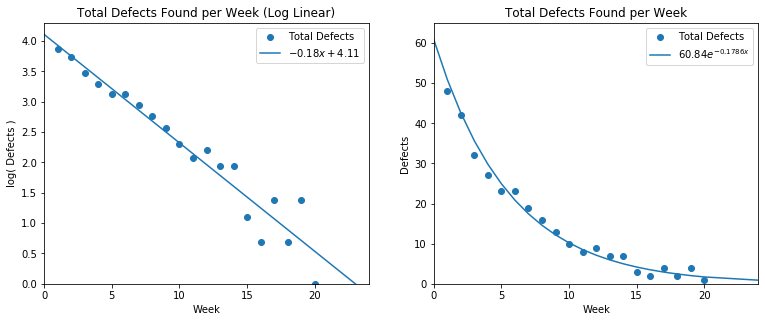
\includegraphics[scale=0.6]{total_log_lin}
			\caption{Defect detection data, total defects log linear regression.}
		\end{figure}
	
		This model fits the data much better than the previous one, with a correlation coefficient of 0.98 and a standard error of 1.72. In other words 98\% of the variation in the total defect finding rate can be explained by this model and standard deviation of the residual error is 1.72.
		
		The total number of defects predicted by this model is approximately 340 ($\int_0^\infty 60.84 e ^ {-0.1786} = 340$) or that there are 40 bugs remaining to be found.
	
	
	\subsection{Total Defects (Non-linear Regression)}
		
		For the third model (figure 4) a non-linear regression was used to calculate the function parameters, and the data's x values were offset by half a week to better reflect the time periods they represent.
		
		Using a non-linear regression results in function with a better fit to the earlier, higher valued data points at the expense of later ones due to a lack of logarithmic scaling in the case of a linear regression.
		
		The other change from the previous model was to shift the dataset back by half a week (i.e. the x values are now 0.5, 1.5, 2.5, ... instead of 1, 2, 3, ...). This was done as while the data records the number of defects found at the end of a given week (previous models' interpretation), they also represent the mean rate of defect finding for that week (this model's interpretation). Offsetting the dataset does not change the goodness of fit as measured by the correlation coefficient or standard error, but it does provide a better model for simulation. A side effect of this alteration is that the predicted defect finding rate and total number of bugs in the system are reduced.
		
		\begin{figure}[hh]
			\centering
			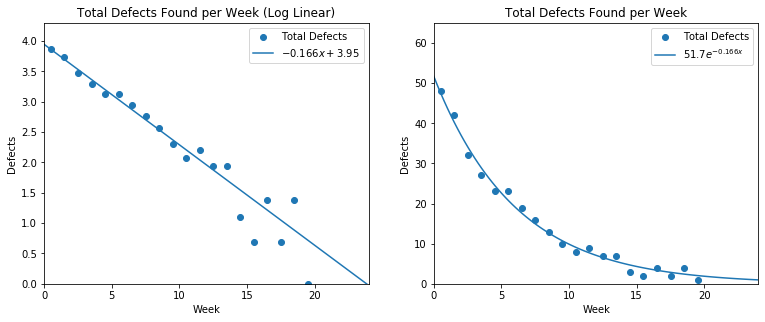
\includegraphics[scale=0.6]{total_nlr}
			\caption{Defect detection data, total defects non linear regression.}
		\end{figure}
	
		There is a slightly improved fit over the previous model with a correlation coefficient of 0.99 and a standard error of 1.4. The area under the curve implies 312 total defects in the system or 12 unfound bugs.
		
	\section{Metrics}
		
% State what metrics you have selected for measuring the maintenance process.

		Four metrics have been chosen to help guide resource allocation strategies for the current project: number of unfound, found and fixed defects; time to fix found defects; impact of unfixed defects and proportion of found defects fixed.
	
	\subsection{Unfound, Found and Fixed Defects}
		This measures the number number of defects that have been found and fixed, those that have been found awaiting fixing and those remaining unfound in the system.
	
	
	\subsection{Time to Fix}
		This measures the time required to fix every found defect in the backlog of bugs waiting to be fixed. Five hours for every hard bug and two hours for every easy bug. This gives the total man hours required to fix every defect that has been found in the system so far.
	
	
	\subsection{Total Impact}
		This measure the impact of all unfixed defects (both found and unfound) on users, based on their statement that ``the major defects are `seven times as damaging' on average as the minor ones''.
	
	
	\subsection{Proportion of Defects Fixed}
		This measures the proportion of defects found that have been fixed, equal to the fixed defects divided by found defects.
	
	
	
	\section{Staff Allocation}
	
% Explain what staff allocation strategy you have selected for your simulation.	
	
		Four staff allocation strategies for finding and fixing bugs have been simulated.
	
	
	\subsection{Strategy One}
		One staff member full-time finding defects, two staff full-time fixing defects. Prioritise fixing defects in the order: major easy, major hard, minor easy, minor hard.
	
	
	\subsection{Strategy Two}
		One staff member full-time finding defects, one staff member full-time fixing defects, one staff member finding defects for ten weeks then fixing defects. Prioritise fixing defects in the order: major easy, major hard, minor easy, minor hard.
	
	
	\subsection{Strategy Three}
		One staff member full-time finding defects, two staff full-time fixing defects. Prioritise fixing defects in the order: major easy, minor easy, major hard, minor hard.


	
	\section{Simulation}

% Describe how you performed your simulations.
% Show the graphs for your metrics for each simulation.
% Identify any assumptions you needed to make, and any limitations in your approach.	
	
	\subsection{Implementation}
		The defect detection and fixing process was simulated using a python script (\texttt{py/sim.py}), it simulates the process of finding and fixing defects hour by hour, with each one of three staff able to allocated to either finding or fixing bugs on a per hour basis. While finding bugs staff make `progress' according to the formula:
	
		\[
			\text{progress} = 2.0661264 e ^ {-0.0066222x}
		\]
	
		This is based on the fitted function from model 3 of the defect detection analysis, scaled to produce a rate of bugs found per hour instead of per week and adjusted very slightly so there are exactly 312 defects in the system. Each hour spent finding defects increases staff progress by an amount determined by the formula, once progress reaches one a bug has is found. When a bug is found the staff's progress is reset to zero and a bug is moved from a pre-randomised list of bugs representing unknown defects to a backlog of found bugs waiting to be fixed. A staff member can be allocated an individual bug to be fixed, once they have been allocated that bug for the requisite time to fix it (two hours for easy and five hours for hard bugs) it is moved from the backlog to fixed bugs.


	\subsection{Assumptions}
	
		Several assumptions are made by the simulation, in particular relating to how testers work and how bugs are found and are listed below:
		\begin{itemize}
			\item All bugs are correctly categorised and fit within each of the four discrete categories.
			\item All bugs are independent, the fixing of one bug will have no impact on any other bugs.
			\item The relative probability of finding different bug types is constant (e.g. there is always a 50\% chance of a bug being a minor easy bug).
			\item Testers are interchangeable, they find and fix bugs at the same rate.
			\item Testers work does not overlap, i.e. two testers won't both find the same bug.
		\end{itemize}
	
	
	\subsection{Limitations}
		
		Some limitations were placed on the simulation, either to increase the ease of implementation or simply due to constraints on the data used.



	\newpage
	\subsection{Metric Graphs}                         

	\begin{figure}[h!]
		\centering
		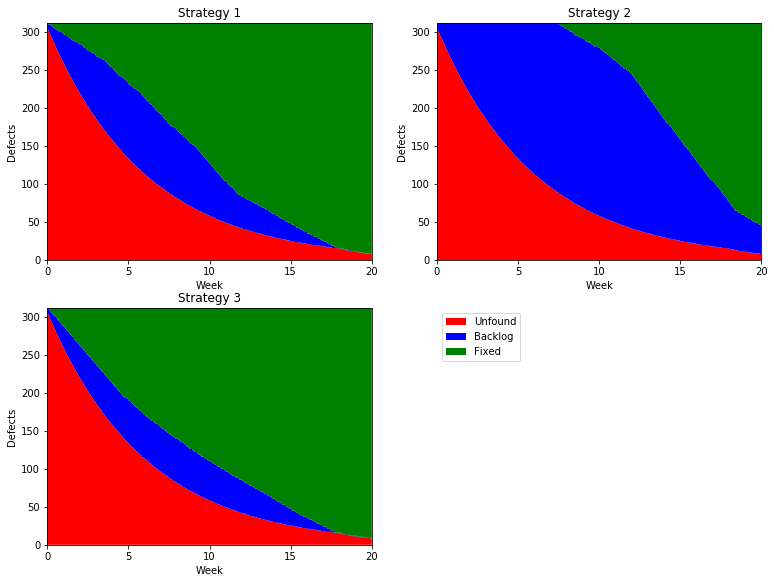
\includegraphics[scale=0.6]{sim_bug_finding}
		\caption{Number of unfound, found and fixed defects for each of the three strategies.}
	\end{figure}

	\begin{center}
		\vspace{4cm}
		[Continued on next page]
	\end{center}

	\begin{figure}[p]
		\centering
		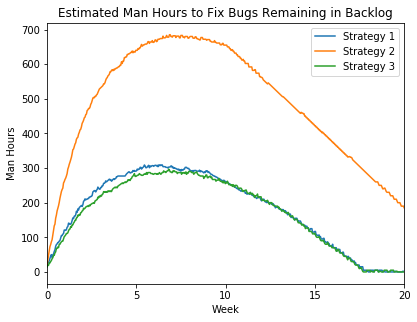
\includegraphics[scale=0.6]{sim_time_to_fix}
		\caption{Estimated time to fix defects that have been found in the system.}
	\end{figure}
	
	\begin{figure}[p]
		\centering
		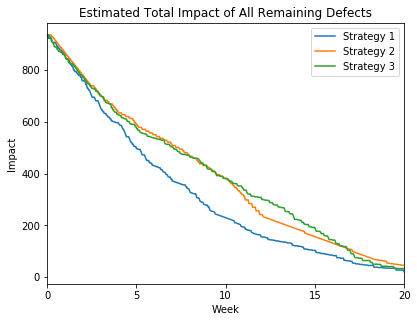
\includegraphics[scale=0.6]{sim_impact}
		\caption{Estimated impact of all unfixed defects remaining in the system.}
	\end{figure}
	
	\begin{figure}[p]
		\centering
		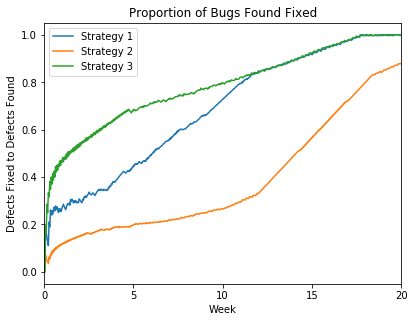
\includegraphics[scale=0.6]{sim_fix_found_proportion}
		\caption{Proportion of defects found that have been fixed.}
	\end{figure}
	\newpage
	
	\section{Discussion}
	
%Relate the results you have found to system reliability and customer satisfaction. Is it possible to state which strategies would result in better reliability or satisfaction? If so, do so. If you wished to minimize the time for which major defects went unfound and unfixed, describe how would you allocate staff.}
	
	The above graphs show the strategies involving one staff member allocated to finding bugs and two to fixing results in defects being fixed sooner on average than the alternative allocation.
	
	Out of the metrics used the best proxy for reliability and customer satisfaction is the impact metric, the others being too abstract (number of bugs unfound, found, fixed and proportion of bugs found fixed) or more relevant more to resource allocation (time to fix). Figure 7 shows how the impact of the defects remaining in the system is reduced, strategy two and three show similar reductions, while the impact of defects is reduced fastest by strategy one.
	
	Lastly, strategy one is also the best of the three for minimising the time major defects go unfound and unfixed. There could be an argument for allocating a second tester to finding for the initial few weeks in order to ensure there are plenty of major defects in the backlog ready to be fixed. However the backlog of found unfixed bug is not cleared until ~90\% of bugs are found and fixed and there is diminishing returns for finding bugs (i.e. the exponential drop off in the defect detection rate). These bot suggest increasing the resource allocated to finding defects, even if only briefly at the start would not reduce major defects' time in the system over staff allocation strategy one.
	

	
	
\end{document}